%=================================================================
% CSE 4345 — Big Data Analytics
% Week 5, Part 1: Handling Big Data Files —
%                 YARN, File Formats, and Optimization
% Department of CSE, Premier University
%
% Part 1 covers: YARN architecture (ResourceManager · NodeManager · ApplicationMaster)
%               · Hadoop 1 vs 2 resource model · Container lifecycle
%               · File formats (CSV · Avro · Parquet · ORC)
%               · Columnar storage benefits · Compression codecs
%               · Splittability · Format selection · Ivy League alignment · Assessment
% Part 2 covers: Vavilapalli et al. (2013) YARN paper · LinkedIn Avro case study
%=================================================================

\documentclass[aspectratio=169,10pt]{beamer}

%---------- Packages ----------
\usepackage[utf8]{inputenc}
\usepackage[T1]{fontenc}
\usepackage{booktabs}
\usepackage{xcolor}
\usepackage{tikz}
\usetikzlibrary{shapes.geometric, positioning, arrows.meta,
                decorations.pathreplacing, calc, fit, backgrounds}
\usepackage{amsmath}
\usepackage{graphicx}
\usepackage{multicol}
\usepackage{enumerate}
\usepackage{array}
\usepackage{listings}

%---------- Theme ----------
\usetheme{Madrid}

%---------- Premier University Color Identity ----------
\definecolor{PUNavy}{RGB}{10,36,99}
\definecolor{PUGold}{RGB}{197,151,37}
\definecolor{PULightBlue}{RGB}{210,228,255}
\definecolor{PUTeal}{RGB}{0,100,100}
\definecolor{PUGray}{RGB}{90,90,90}
\definecolor{PURed}{RGB}{160,30,30}
\definecolor{PUGreen}{RGB}{30,120,60}
\definecolor{PUOrange}{RGB}{200,100,20}
\definecolor{PUPurple}{RGB}{80,0,120}

\setbeamercolor{palette primary}{bg=PUNavy, fg=white}
\setbeamercolor{palette secondary}{bg=PUNavy!85, fg=white}
\setbeamercolor{palette tertiary}{bg=PUNavy!70, fg=white}
\setbeamercolor{palette quaternary}{bg=PUNavy, fg=white}
\setbeamercolor{structure}{fg=PUNavy}
\setbeamercolor{title}{bg=PUNavy, fg=PUGold}
\setbeamercolor{subtitle}{fg=white}
\setbeamercolor{frametitle}{bg=PUNavy, fg=PUGold}
\setbeamercolor{alerted text}{fg=PUGold!85!black}
\setbeamercolor{block title}{bg=PUNavy, fg=white}
\setbeamercolor{block body}{bg=PULightBlue!45}
\setbeamercolor{block title alerted}{bg=PUGold!80!black, fg=white}
\setbeamercolor{block body alerted}{bg=PUGold!12}
\setbeamercolor{block title example}{bg=PUTeal, fg=white}
\setbeamercolor{block body example}{bg=PUTeal!10}
\setbeamercolor{section in toc}{fg=PUNavy}
\setbeamercolor{itemize item}{fg=PUGold!80!black}
\setbeamercolor{itemize subitem}{fg=PUNavy!70}

\setbeamertemplate{navigation symbols}{}
\setbeamertemplate{itemize item}{\scriptsize\raise1.5pt\hbox{\textbullet}}
\setbeamertemplate{itemize subitem}{\scriptsize\raise1pt\hbox{--}}

%---------- Code listing style ----------
\lstset{
  basicstyle=\ttfamily\scriptsize,
  backgroundcolor=\color{PUNavy!8},
  frame=single,
  rulecolor=\color{PUNavy!30},
  breaklines=true,
  language={},
}

%---------- Section separator ----------
\AtBeginSection[]{
  \begin{frame}[plain]
    \vfill\centering
    \begin{beamercolorbox}[sep=12pt,center,shadow=true,rounded=true]{block title}
      \usebeamerfont{title}\insertsectionhead\par
    \end{beamercolorbox}
    \vfill
  \end{frame}
}

%---------- Title metadata ----------
\title[CSE 4345 \textbar{} Week 5, Part 1]{CSE 4345: Big Data Analytics}
\subtitle{Week 5, Part 1 \textemdash\ Handling Big Data Files:
          YARN, File Formats \& Optimization}
\author[Dept.\ of CSE]{Department of Computer Science \& Engineering\\[4pt]
       \small Premier University, Chittagong}
\institute{}
\date{Semester 2026}

%=================================================================
\begin{document}
%=================================================================

%----------------------------------------------------------------
% TITLE SLIDE
%----------------------------------------------------------------
\begin{frame}
  \titlepage
\end{frame}

%----------------------------------------------------------------
% COURSE INFO
%----------------------------------------------------------------
\begin{frame}{Course \& Lecture Information}
  \begin{columns}[T]
    \column{0.47\textwidth}
      \begin{block}{Lecture Identity}
        \begin{tabular}{ll}
          \textbf{Course:}      & CSE 4345 \\
          \textbf{Week / Part:} & 5 of 11 \textbar\ Part 1 of 2 \\
          \textbf{CLO:}         & CLO3 \\
          \textbf{PLO:}         & PLO(e), PLO(f) \\
        \end{tabular}
      \end{block}
      \vspace{6pt}
      \begin{alertblock}{CLO3}
        \textit{``Explain big data techniques, tools, and technologies used to store, manage, and analyse large datasets''}
      \end{alertblock}
      \vspace{6pt}
      \begin{block}{Course Progression}
        \small
        Week 3: HDFS (where data lives)\\
        Week 4: MapReduce / Pig / Hive / HBase (how data is processed)\\
        \textbf{Week 5: How data is \emph{formatted, compressed, scheduled}}\\
        Week 6: Apache Spark (in-memory computing)
      \end{block}

    \column{0.50\textwidth}
      \begin{exampleblock}{Part 1 Covers}
        \begin{itemize}
          \item Why storage format and scheduling matter at scale
          \item Hadoop 1.x vs.\ Hadoop 2.x: the YARN revolution
          \item YARN three-component architecture
          \item Container lifecycle and job execution flow
          \item File formats: CSV/Text, Avro, Parquet, ORC
          \item Row-oriented vs.\ columnar storage (why it matters)
          \item Compression codecs: Snappy, Gzip, LZO, Zstd
          \item Splittability: the critical property
          \item Format selection matrix for production
          \item Ivy League alignment
          \item Student assessment pool
        \end{itemize}
      \end{exampleblock}
  \end{columns}
\end{frame}

%----------------------------------------------------------------
\begin{frame}{Lecture Agenda}
  \tableofcontents
\end{frame}

%================================================================
\section{The Storage \& Scheduling Problem}
%================================================================

\begin{frame}{Why Format and Scheduling Matter}
  \begin{columns}[T]
    \column{0.52\textwidth}
      \begin{block}{The Two Questions After HDFS \& MapReduce}
        Once we can \emph{store} data (HDFS) and \emph{compute} over it (MapReduce), two engineering questions dominate production performance:
        \vspace{4pt}
        \begin{enumerate}
          \item \textbf{Scheduling:} How do we share a 1{,}000-node cluster across 50 simultaneous jobs, different teams, and different frameworks (MapReduce, Spark, Tez) — fairly and efficiently?
          \item \textbf{Format:} How do we store data so that a query reading 3 of 100 columns reads 3\% of the data, not 100\%?
        \end{enumerate}
      \end{block}
      \vspace{4pt}
      \begin{exampleblock}{Real Cost at Scale}
        \small A 100-column table with 10 TB of data. A query selects 3 columns:
        \begin{itemize}
          \item \textbf{CSV (row store):} reads all 10 TB
          \item \textbf{Parquet (column store):} reads $\approx$300 GB
          \item \textbf{Speedup: $33\times$} from format alone
        \end{itemize}
      \end{exampleblock}

    \column{0.45\textwidth}
      \begin{alertblock}{Hadoop 1.x Bottleneck}
        In Hadoop 1.x, MapReduce v1 bundled resource management with computation. Every cluster resource was managed by the \textbf{JobTracker}, which:
        \vspace{4pt}
        \begin{itemize}
          \item Only ran MapReduce jobs (Spark, Tez, Storm had no path to cluster resources)
          \item Had a single JobTracker as a bottleneck ($\approx$4{,}000 node limit)
          \item Mixed cluster scheduling with job coordination
        \end{itemize}
        \vspace{4pt}
        \textbf{The fix:} Separate resource management from computation. This became \textbf{YARN} in Hadoop 2.0 (2013).
      \end{alertblock}
  \end{columns}
\end{frame}

%================================================================
\section{YARN: The Resource Management Revolution}
%================================================================

\begin{frame}{Hadoop 1 vs.\ Hadoop 2: The YARN Split}
  \begin{center}
  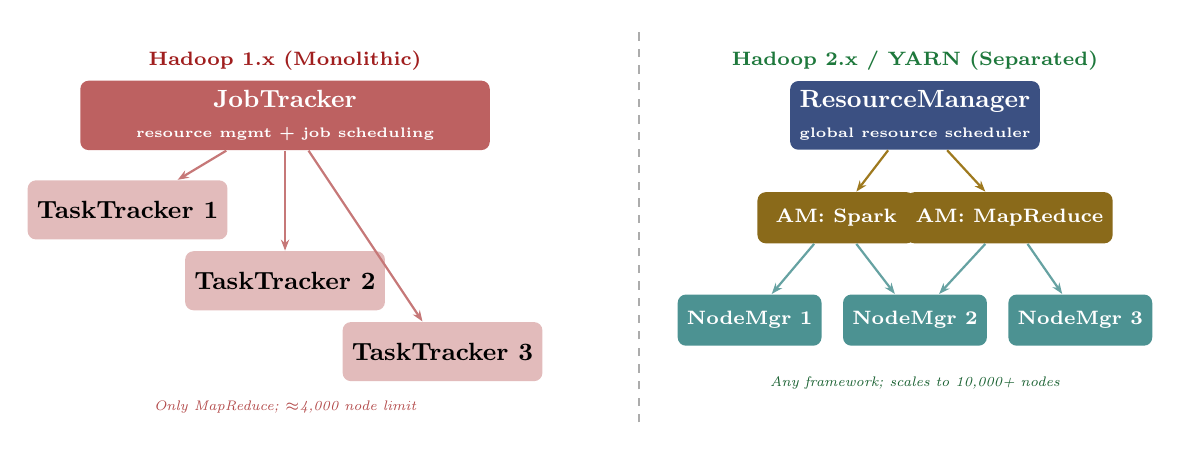
\begin{tikzpicture}[
      box/.style={rectangle, rounded corners=3pt,
                  minimum width=2.6cm, minimum height=0.75cm,
                  align=center, font=\small\bfseries},
      arr/.style={-{Stealth[length=4pt]}, thick},
      lbl/.style={font=\scriptsize\bfseries}
    ]

    %--- Hadoop 1.x (left) ---
    \node[lbl, PURed] at (-4.5, 3.8) {Hadoop 1.x (Monolithic)};

    \node[box, fill=PURed!70, text=white, minimum width=5.2cm]
          (jt) at (-4.5, 3.1) {JobTracker\\{\tiny resource mgmt + job scheduling}};
    \foreach \i/\y/\xx in {1/1.9/-6.5, 2/1.0/-4.5, 3/0.1/-2.5} {
      \node[box, fill=PURed!30, minimum width=2.0cm]
            (tt\i) at (\xx, \y) {TaskTracker \i};
      \draw[arr, PURed!60] (jt) -- (tt\i);
    }
    \node[font=\tiny\itshape, PURed!80] at (-4.5,-0.6)
          {Only MapReduce; $\approx$4{,}000 node limit};

    %--- Hadoop 2.x (right) ---
    \node[lbl, PUGreen] at (3.5, 3.8) {Hadoop 2.x / YARN (Separated)};

    \node[box, fill=PUNavy!80, text=white, minimum width=3.0cm]
          (rm) at (3.5, 3.1) {ResourceManager\\{\tiny global resource scheduler}};

    \foreach \i/\y/\lbl/\xx in {1/1.8/Spark/2.5, 2/1.8/MapReduce/4.7} {
      \node[box, fill=PUGold!70!black, text=white, minimum width=2.0cm,
            minimum height=0.65cm, font=\scriptsize\bfseries]
            (am\i) at (\xx, \y) {AM: \lbl};
      \draw[arr, PUGold!80!black] (rm) -- (am\i);
    }

    \foreach \i/\x in {1/1.4, 2/3.5, 3/5.6} {
      \node[box, fill=PUTeal!70, text=white, minimum width=1.6cm,
            minimum height=0.65cm, font=\scriptsize\bfseries]
            (nm\i) at (\x, 0.5) {NodeMgr \i};
    }
    \draw[arr, PUTeal!60] (am1) -- (nm1);
    \draw[arr, PUTeal!60] (am1) -- (nm2);
    \draw[arr, PUTeal!60] (am2) -- (nm2);
    \draw[arr, PUTeal!60] (am2) -- (nm3);

    \node[font=\tiny\itshape, PUGreen!80!black] at (3.5,-0.3)
          {Any framework; scales to 10{,}000+ nodes};

    %--- Divider ---
    \draw[thick, PUGray!50, dashed] (0, -0.8) -- (0, 4.2);
  \end{tikzpicture}
  \end{center}
  \vspace{2pt}
  \begin{alertblock}{The Key Architectural Decision}
    YARN introduced the \textbf{ApplicationMaster} — a per-job component that \emph{negotiates} resources from the ResourceManager.  This decoupling means any framework (Spark, Flink, Tez) can run on a YARN cluster without knowing how the cluster scheduler works.
  \end{alertblock}
\end{frame}

%----------------------------------------------------------------
\begin{frame}{YARN Three-Component Architecture}
  \begin{columns}[T]
    \column{0.45\textwidth}
      \begin{block}{1. ResourceManager (RM)}
        Global cluster resource scheduler.  Runs on a dedicated master node.
        \begin{itemize}
          \item \textbf{Scheduler}: allocates \emph{containers} to ApplicationMasters; pluggable (FIFO, Fair, Capacity)
          \item \textbf{ApplicationsManager}: accepts job submissions; starts the first container for each ApplicationMaster
        \end{itemize}
      \end{block}
      \vspace{4pt}
      \begin{block}{2. NodeManager (NM)}
        Per-node agent running on every worker node.
        \begin{itemize}
          \item Launches and monitors \textbf{containers} on the local machine
          \item Reports node health and container status to RM via heartbeat
          \item Manages local resource isolation (CPU, RAM, disk I/O limits per container)
        \end{itemize}
      \end{block}

    \column{0.52\textwidth}
      \begin{exampleblock}{3. ApplicationMaster (AM)}
        One per running job — the job's own scheduler.
        \begin{itemize}
          \item Requests resources (containers) from the RM on behalf of the job
          \item Tells the NM to launch specific tasks inside those containers
          \item Monitors task progress; re-requests containers for failed tasks
          \item Releases containers when tasks complete
        \end{itemize}
        \vspace{4pt}
        \textbf{Example:} A Spark AM requests 100 containers (each 4 cores, 8 GB RAM) for Spark Executors; the RM grants 80 (cluster is busy); the AM assigns tasks to those 80 Executors.
      \end{exampleblock}
      \vspace{4pt}
      \begin{alertblock}{Container = Resource Slice}
        A \textbf{container} is an abstract unit of cluster capacity: a specific number of CPU cores + a specific amount of RAM, allocated from one NodeManager.  Tasks run inside containers.
      \end{alertblock}
  \end{columns}
\end{frame}

%----------------------------------------------------------------
\begin{frame}{YARN Job Execution Flow}
  \begin{center}
  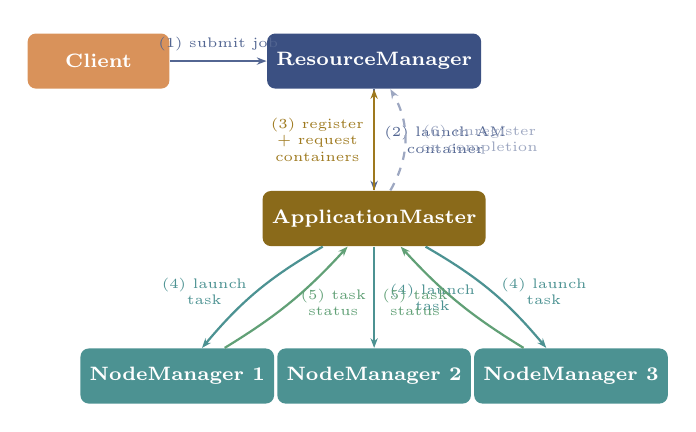
\begin{tikzpicture}[
      actor/.style={rectangle, rounded corners=3pt,
                    minimum width=1.8cm, minimum height=0.7cm,
                    font=\scriptsize\bfseries, align=center},
      arr/.style={-{Stealth[length=3.5pt]}, thick},
      lbl/.style={font=\tiny, align=center}
    ]
    \node[actor, fill=PUOrange!70, text=white]  (cl)  at (0,   5.5) {Client};
    \node[actor, fill=PUNavy!80,    text=white]  (rm)  at (3.5, 5.5) {ResourceManager};
    \node[actor, fill=PUGold!70!black, text=white] (am)  at (3.5, 3.5) {ApplicationMaster};
    \node[actor, fill=PUTeal!70,    text=white]  (nm1) at (1.0, 1.5) {NodeManager 1};
    \node[actor, fill=PUTeal!70,    text=white]  (nm2) at (3.5, 1.5) {NodeManager 2};
    \node[actor, fill=PUTeal!70,    text=white]  (nm3) at (6.0, 1.5) {NodeManager 3};

    % Step arrows
    \draw[arr, PUNavy!70]    (cl)  -- node[above, lbl]{(1) submit job} (rm);
    \draw[arr, PUNavy!70]    (rm)  -- node[right, lbl]{(2) launch AM\\container} (am);
    \draw[arr, PUGold!80!black] (am) -- node[left,  lbl]{(3) register\\ + request\\containers} (rm);
    \draw[arr, PUTeal!70]    (am)  to[bend right=10] node[lbl,left]{(4) launch\\task} (nm1);
    \draw[arr, PUTeal!70]    (am)  -- node[lbl,right,xshift=2pt]{(4) launch\\task} (nm2);
    \draw[arr, PUTeal!70]    (am)  to[bend left=10]  node[lbl,right]{(4) launch\\task} (nm3);
    \draw[arr, PUGreen!70]   (nm1) to[bend right=8] node[lbl,right]{(5) task\\status} (am);
    \draw[arr, PUGreen!70]   (nm3) to[bend left=8]  node[lbl,left]{(5) task\\status} (am);
    \draw[arr, PUNavy!40, dashed] (am) to[bend right=30]
          node[lbl, right, xshift=2pt]{(6) unregister\\on completion} (rm);
  \end{tikzpicture}
  \end{center}
  \vspace{2pt}
  \begin{block}{YARN Fault Tolerance}
    \small If a \textbf{NodeManager fails}, the RM detects via missed heartbeats and marks all containers on that node as failed; the AM re-requests replacement containers.  If the \textbf{AM itself fails}, the RM can restart a new AM (configured via \texttt{yarn.resourcemanager.am.max-attempts}).
  \end{block}
\end{frame}

%----------------------------------------------------------------
\begin{frame}{YARN Schedulers: Sharing the Cluster}
  \begin{columns}[T]
    \column{0.52\textwidth}
      \begin{block}{Three Built-in Scheduler Policies}
        \vspace{4pt}
        \begin{enumerate}
          \item \textbf{FIFO Scheduler}: jobs run in submission order; simple but not suitable for multi-tenant clusters (one long job starves all others)
          \item \textbf{Capacity Scheduler} (default in HDP/CDH): cluster divided into queues with guaranteed capacity; e.g., Engineering queue = 60\%, Finance queue = 40\%; elastically borrows unused capacity
          \item \textbf{Fair Scheduler} (default in Cloudera): all jobs get equal share of resources; latency-sensitive short jobs complete quickly even if a large job is running
        \end{enumerate}
      \end{block}

    \column{0.45\textwidth}
      \begin{exampleblock}{Bangladesh Context: a2i Cluster Sharing}
        \small The a2i (Access to Information) programme runs analytics on government data:
        \vspace{4pt}
        \begin{itemize}
          \item \textbf{Queue A (60\%)}: nightly DGHS health-record batch jobs (MapReduce)
          \item \textbf{Queue B (30\%)}: Spark streaming for real-time agriculture data from DAE
          \item \textbf{Queue C (10\%)}: ad-hoc Hive queries by data analysts
        \end{itemize}
        \vspace{4pt}
        With \textbf{Capacity Scheduler}, queue B cannot monopolise resources even during peak streaming periods; queue A is guaranteed its 60\%.
      \end{exampleblock}
      \vspace{4pt}
      \begin{alertblock}{DRF: Dominant Resource Fairness}
        \small In a heterogeneous cluster (CPU-heavy vs.\ RAM-heavy jobs), YARN uses \textbf{DRF} (Ghodsi et al., 2011) to define fairness across multiple resource dimensions — not just memory.
      \end{alertblock}
  \end{columns}
\end{frame}

%================================================================
\section{File Formats: Row vs.\ Columnar Storage}
%================================================================

\begin{frame}{The Row vs.\ Columnar Storage Fundamental}
  \begin{center}
  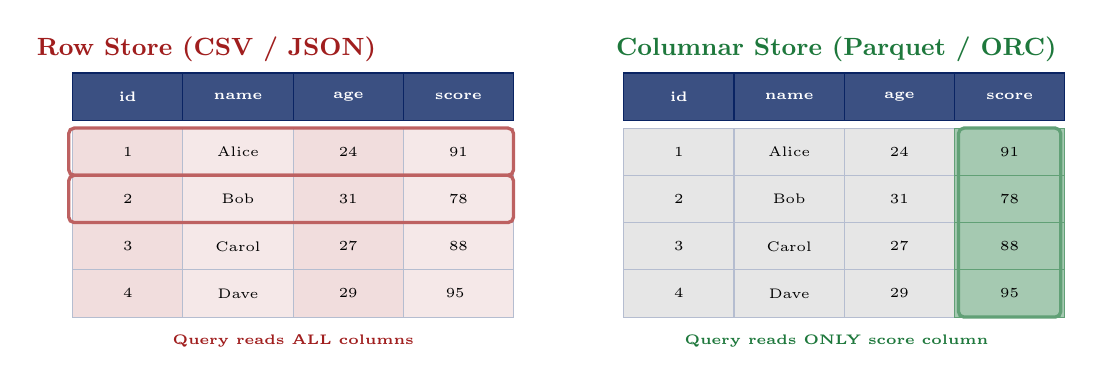
\begin{tikzpicture}[
      cell/.style={rectangle, draw=PUNavy!30, minimum width=1.4cm,
                   minimum height=0.6cm, font=\tiny, align=center},
      hdr/.style={rectangle, fill=PUNavy!80, text=white, draw=PUNavy,
                  minimum width=1.4cm, minimum height=0.6cm,
                  font=\tiny\bfseries, align=center}
    ]

    %--- Row store (left) ---
    \node[font=\small\bfseries, PURed] at (-4.5, 3.8) {Row Store (CSV / JSON)};
    \foreach \c/\x in {id/-5.5, name/-4.1, age/-2.7, score/-1.3} {
      \node[hdr] at (\x, 3.2) {\c};
    }
    \foreach \r/\y/\cola/\colb/\colc/\cold in {
      1/2.5/1/Alice/24/91,
      2/1.9/2/Bob/31/78,
      3/1.3/3/Carol/27/88,
      4/0.7/4/Dave/29/95
    } {
      \node[cell, fill=PURed!15]  at (-5.5,\y) {\cola};
      \node[cell, fill=PURed!10]  at (-4.1,\y) {\colb};
      \node[cell, fill=PURed!15]  at (-2.7,\y) {\colc};
      \node[cell, fill=PURed!10]  at (-1.3,\y) {\cold};
    }
    % Highlight entire rows (read all)
    \draw[PURed!70, very thick, rounded corners=2pt]
          (-6.25,2.2) rectangle (-0.6,2.8);
    \draw[PURed!70, very thick, rounded corners=2pt]
          (-6.25,1.6) rectangle (-0.6,2.2);
    \node[font=\tiny\bfseries, PURed] at (-3.4, 0.1)
          {Query reads ALL columns};

    %--- Columnar store (right) ---
    \node[font=\small\bfseries, PUGreen] at (3.5, 3.8) {Columnar Store (Parquet / ORC)};
    \foreach \c/\x in {id/1.5, name/2.9, age/4.3, score/5.7} {
      \node[hdr] at (\x, 3.2) {\c};
    }
    % Data stored column by column
    \foreach \val/\y in {1/2.5, 2/1.9, 3/1.3, 4/0.7} {
      \node[cell, fill=PUGray!15] at (1.5,\y) {\val};
    }
    \foreach \val/\y in {Alice/2.5, Bob/1.9, Carol/1.3, Dave/0.7} {
      \node[cell, fill=PUGray!15] at (2.9,\y) {\val};
    }
    \foreach \val/\y in {24/2.5, 31/1.9, 27/1.3, 29/0.7} {
      \node[cell, fill=PUGray!15] at (4.3,\y) {\val};
    }
    % Highlight ONLY score column
    \foreach \val/\y in {91/2.5, 78/1.9, 88/1.3, 95/0.7} {
      \node[cell, fill=PUGreen!40, draw=PUGreen!70] at (5.7,\y) {\val};
    }
    \draw[PUGreen!70, very thick, rounded corners=2pt]
          (5.05,0.4) rectangle (6.35,2.8);
    \node[font=\tiny\bfseries, PUGreen] at (3.5, 0.1)
          {Query reads ONLY score column};
  \end{tikzpicture}
  \end{center}
  \vspace{2pt}
  \begin{alertblock}{I/O Reduction at Scale}
    \small \textbf{Row store}: \texttt{SELECT score FROM users} reads ALL columns (id, name, age, score).  \textbf{Columnar store}: reads ONLY the score column — physically skipping id, name, age on disk.  For a 100-column table, this is a \textbf{97\% I/O reduction} for a 3-column query.
  \end{alertblock}
\end{frame}

%----------------------------------------------------------------
\begin{frame}{File Format Deep Dive: Avro, Parquet, ORC}
  \centering
  \renewcommand{\arraystretch}{1.45}
  \begin{tabular}{p{1.6cm}p{1.5cm}p{1.7cm}p{1.5cm}p{1.5cm}p{3.0cm}}
    \toprule
    \textbf{Format} & \textbf{Orientation} & \textbf{Schema} & \textbf{Splittable} & \textbf{Compression} & \textbf{Best For} \\
    \midrule
    \textbf{Text / CSV}
      & Row & External & With codec & None (default) & Portability, small data \\
    \textbf{JSON (lines)}
      & Row & Self & No (raw) & External & APIs, log ingestion \\
    \textbf{Avro}
      & Row & Self-describing (JSON) & Yes & Snappy/Deflate & Schema evolution, Kafka $\to$ HDFS \\
    \textbf{Parquet}
      & Columnar & Self-describing & Yes & Snappy/Gzip & Spark, Presto, ML pipelines \\
    \textbf{ORC}
      & Columnar & Self-describing & Yes & Zlib/Snappy & Hive, highest compression \\
    \bottomrule
  \end{tabular}
  \vspace{8pt}
  \begin{columns}[T]
    \column{0.48\textwidth}
      \begin{block}{Why Avro for Schema Evolution?}
        \small When LinkedIn adds a new field to a Kafka event schema, old consumers reading the same HDFS files must not break.  Avro's \textbf{reader schema vs.\ writer schema} protocol allows backward and forward compatibility: missing fields use default values; extra fields are ignored.
      \end{block}
    \column{0.48\textwidth}
      \begin{alertblock}{Why Parquet for Analytics?}
        \small Parquet stores data in \textbf{row groups} ($\sim$128 MB each) which contain \textbf{column chunks}.  Statistics (min/max per column chunk) enable \textbf{predicate pushdown}: skip entire row groups where \texttt{score < 80} without reading them.
      \end{alertblock}
  \end{columns}
\end{frame}

%================================================================
\section{Compression Codecs \& Splittability}
%================================================================

\begin{frame}{Compression Codecs: The Trade-off Landscape}
  \begin{columns}[T]
    \column{0.50\textwidth}
      \begin{block}{Key Compression Codecs in Hadoop}
        \renewcommand{\arraystretch}{1.3}
        \begin{tabular}{p{1.4cm}p{1.1cm}p{1.0cm}p{1.6cm}}
          \toprule
          \textbf{Codec} & \textbf{Speed} & \textbf{Ratio} & \textbf{Splittable?} \\
          \midrule
          Snappy & Fast & Medium & No (but Parquet row groups are) \\
          Gzip   & Slow & High   & \alert{No} \\
          LZO    & Fast & Medium & Yes (with index) \\
          Bzip2  & Slowest & Highest & Yes \\
          Zstd   & Fast & High   & No (block-level) \\
          \bottomrule
        \end{tabular}
      \end{block}
      \vspace{6pt}
      \begin{alertblock}{The Gzip Trap — Very Common Mistake}
        Gzip is \textbf{NOT splittable}.  A 10 GB gzip-compressed CSV file is processed by \textbf{exactly 1 Mapper} — no parallelism.  HDFS stores it in blocks, but MapReduce cannot split across gzip boundaries.  \textbf{Solution:} use Parquet+Snappy (splittable at row-group boundaries) or bzip2 (natively splittable).
      \end{alertblock}

    \column{0.47\textwidth}
      \begin{exampleblock}{What Does ``Splittable'' Mean?}
        A file format is \textbf{splittable} if HDFS can start reading from any point in the file without needing to decompress from the beginning.
        \vspace{6pt}
        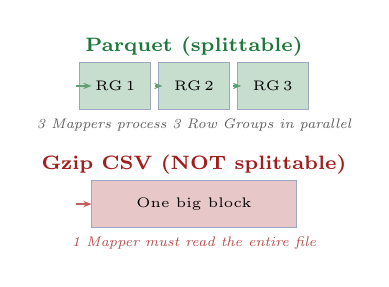
\begin{tikzpicture}[
            blk/.style={rectangle, draw=PUNavy!40, minimum width=0.9cm,
                        minimum height=0.6cm, font=\tiny, align=center},
            arr/.style={-{Stealth[length=3pt]}, thick}
          ]
          % Parquet (splittable)
          \node[font=\scriptsize\bfseries, PUGreen] at (1.3, 2.4) {Parquet (splittable)};
          \foreach \i/\x in {1/0.3, 2/1.3, 3/2.3} {
            \node[blk, fill=PUGreen!25] (p\i) at (\x, 1.9) {RG\,\i};
          }
          \draw[arr, PUGreen!70] (-0.2, 1.9) -- (0.0, 1.9);
          \draw[arr, PUGreen!70]  (0.8, 1.9) -- (0.9, 1.9);
          \draw[arr, PUGreen!70]  (1.8, 1.9) -- (1.9, 1.9);
          \node[font=\tiny\itshape, PUGray] at (1.3, 1.4)
                {3 Mappers process 3 Row Groups in parallel};

          % Gzip (not splittable)
          \node[font=\scriptsize\bfseries, PURed] at (1.3, 0.9) {Gzip CSV (NOT splittable)};
          \node[blk, fill=PURed!25, minimum width=2.6cm]
                at (1.3, 0.4) {One big block};
          \draw[arr, PURed!70] (-0.2, 0.4) -- (0.0, 0.4);
          \node[font=\tiny\itshape, PURed!80] at (1.3, -0.1)
                {1 Mapper must read the entire file};
        \end{tikzpicture}
      \end{exampleblock}
      \vspace{4pt}
      \begin{block}{Best Practice}
        \small Use \textbf{Parquet + Snappy} for analytics (Spark, Hive).  Use \textbf{Avro + Snappy} for streaming ingest (Kafka $\to$ HDFS).  Avoid raw gzip on large CSV files.
      \end{block}
  \end{columns}
\end{frame}

%----------------------------------------------------------------
\begin{frame}{Inside Parquet: Row Groups, Column Chunks, Pages}
  \begin{columns}[T]
    \column{0.50\textwidth}
      \begin{block}{Parquet Internal Layout}
        \vspace{4pt}
        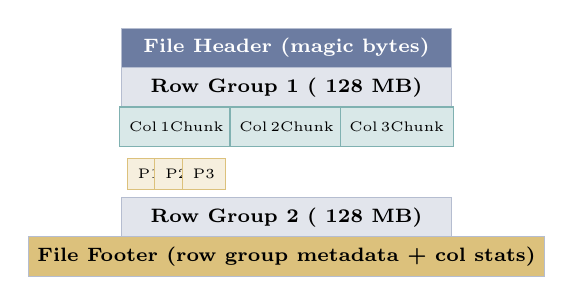
\begin{tikzpicture}[
            outer/.style={rectangle, draw=PUNavy!40, rounded corners=3pt,
                          minimum width=4.5cm, align=center},
            rg/.style={rectangle, fill=PUNavy!12, draw=PUNavy!30,
                       minimum width=4.2cm, minimum height=0.5cm,
                       font=\scriptsize\bfseries, align=center},
            cc/.style={rectangle, draw=PUTeal!50, fill=PUTeal!15,
                       minimum width=1.3cm, minimum height=0.5cm,
                       font=\tiny, align=center},
            pg/.style={rectangle, draw=PUGold!60, fill=PUGold!15,
                       minimum width=0.55cm, minimum height=0.4cm,
                       font=\tiny, align=center}
          ]
          % File header
          \node[rg, fill=PUNavy!60, text=white] at (0, 3.5) {File Header (magic bytes)};
          % Row group 1
          \node[rg] at (0, 3.0) {Row Group 1 (~128 MB)};
          \foreach \i/\x in {1/-1.4, 2/0, 3/1.4} {
            \node[cc] (cc\i) at (\x, 2.5) {Col\,\i Chunk};
          }
          % Pages inside col chunk
          \foreach \j/\x in {1/-1.75, 2/-1.4, 3/-1.05} {
            \node[pg] at (\x, 1.9) {P\j};
          }
          % Row group 2
          \node[rg] at (0, 1.35) {Row Group 2 (~128 MB)};
          % Footer
          \node[rg, fill=PUGold!60] at (0, 0.85) {File Footer (row group metadata + col stats)};
        \end{tikzpicture}
      \end{block}

    \column{0.47\textwidth}
      \begin{exampleblock}{Why This Layout Enables Predicate Pushdown}
        \small
        \textbf{Query:} \texttt{WHERE score > 90}
        \vspace{4pt}
        \begin{enumerate}
          \item Read \textbf{File Footer} only: get column stats (min/max) per row group per column chunk
          \item Row Group 1 has score in [60, 85] $\to$ \textbf{skip entire row group} (no I/O)
          \item Row Group 2 has score in [85, 99] $\to$ must read this chunk
          \item Within Row Group 2: read only the \textbf{score column chunk}
        \end{enumerate}
        \vspace{4pt}
        $\Rightarrow$ A query on 10 TB Parquet may physically read only \textbf{50 GB}.
      \end{exampleblock}
      \vspace{4pt}
      \begin{alertblock}{Parquet + Spark}
        \small Spark natively reads Parquet with predicate pushdown enabled by default (\texttt{spark.sql.parquet.filterPushdown=true}).  No configuration needed — the performance gain is automatic.
      \end{alertblock}
  \end{columns}
\end{frame}

%================================================================
\section{Format Selection in Production}
%================================================================

\begin{frame}{Format Selection Decision Matrix}
  \begin{center}
  \renewcommand{\arraystretch}{1.5}
  \begin{tabular}{p{3.5cm}p{2.4cm}p{2.5cm}p{2.8cm}}
    \toprule
    \textbf{Scenario} & \textbf{Recommended Format} & \textbf{Compression} & \textbf{Reason} \\
    \midrule
    Streaming ingest (Kafka $\to$ HDFS)
      & Avro & Snappy & Schema evolution; row-append friendly \\
    Spark analytics pipeline
      & Parquet & Snappy & Columnar; predicate pushdown; Spark native \\
    Hive SQL warehouse
      & ORC & Zlib & Best compression; Hive ACID support; vectorized reads \\
    Data exchange / APIs
      & Avro or JSON & None & Human-readable schema; broad ecosystem support \\
    Machine learning features
      & Parquet & Gzip & Column-oriented; Scikit-learn / TensorFlow readers exist \\
    Archive / cold storage
      & ORC or Parquet & Zstd & Highest compression; long-term cost reduction \\
    \midrule
    \textbf{AVOID}
      & CSV+Gzip & Gzip & Not splittable; poor analytics performance \\
    \bottomrule
  \end{tabular}
  \end{center}
  \vspace{4pt}
  \begin{block}{Bangladesh Context: bKash Data Lake Format Strategy}
    \small \textbf{Ingest layer}: Kafka events $\to$ Avro (schema evolution for API versioning).
    \textbf{Analytics layer}: convert nightly to Parquet+Snappy (partitioned by \texttt{dt=YYYY-MM-DD/region=}).
    \textbf{Archive}: cold data $>$2 years $\to$ ORC+Zstd (60\% size reduction vs.\ CSV).
  \end{block}
\end{frame}

%================================================================
\section{Ivy League Alignment}
%================================================================

\begin{frame}{YARN \& File Formats in Top University Curricula}
  \begin{columns}[T]
    \column{0.55\textwidth}
      \begin{block}{Harvard CS265 — Big Data Systems (Idreos)}
        \small Harvard frames file formats as a \textbf{fundamental algorithm design decision}:
        \begin{itemize}
          \item \textbf{I/O complexity model}: the cost of an algorithm is measured in the number of \emph{I/O operations} (not time), and columnar formats directly reduce this measure
          \item \textbf{Access path selection}: just as a database optimizer chooses between a full table scan and an index, Parquet's predicate pushdown acts as a \emph{lightweight index} embedded in the footer
          \item Harvard's benchmark: Parquet with predicate pushdown reduces I/O by $10$--$100\times$ for selective queries on wide tables (100+ columns)
        \end{itemize}
        \textbf{Harvard exam question:} \textit{``Prove that for a query selecting $k$ columns from a $c$-column row-store table of $n$ rows, the I/O complexity is $\Theta(n \cdot c)$, but $\Theta(n \cdot k)$ for a column store.''}
      \end{block}

    \column{0.42\textwidth}
      \begin{exampleblock}{MIT 6.830 — Database Systems}
        \small MIT compares YARN's DRF scheduler with classical database concurrency control:
        \begin{itemize}
          \item \textbf{DRF} (Ghodsi et al., 2011): generalises max-min fairness to multiple resource dimensions — the dominant resource of a job determines its fair share
          \item The YARN Capacity Scheduler is a practical implementation of hierarchical DRF with preemption
        \end{itemize}
      \end{exampleblock}
      \vspace{4pt}
      \begin{alertblock}{CMU 15-721 — Advanced DB Systems}
        \small CMU covers Parquet/ORC as modern implementations of the \textbf{DSM (Decomposition Storage Model)} — column stores first formalised by Copeland \& Khoshafian (1985).  Predicate pushdown and late materialisation in Parquet match the techniques used in commercial column stores (Vertica, Snowflake).
      \end{alertblock}
  \end{columns}
\end{frame}

%================================================================
\section{Student Assessment Pool}
%================================================================

\begin{frame}{Assessment\textemdash MCQ Set A \hfill\small\textit{CLO3}}
  \begin{exampleblock}{Instructions}
    Select the single best answer.  Correct answers \textbf{bolded} for instructor reference.
  \end{exampleblock}
  \vspace{8pt}
  \begin{itemize}
    \item[\textbf{Q1.}] Which component in YARN is responsible for \textbf{global resource allocation} across the entire cluster?
    \begin{enumerate}[(a)]
      \item NodeManager \quad (b) ApplicationMaster \quad (c) \textbf{ResourceManager} \quad (d) NameNode
    \end{enumerate}
  \end{itemize}
  \vspace{8pt}
  \begin{itemize}
    \item[\textbf{Q2.}] Which Hadoop file format stores data in \textbf{columnar} format and is best suited for analytical, read-heavy workloads?
    \begin{enumerate}[(a)]
      \item Avro \quad (b) Text/CSV \quad (c) \textbf{Parquet} \quad (d) JSON
    \end{enumerate}
  \end{itemize}
  \vspace{8pt}
  \begin{alertblock}{Instructor Notes}
    \textbf{Q1:} Students confuse ApplicationMaster (per-job) with ResourceManager (global).  Reinforce: \textbf{one RM per cluster}, one AM per running application.  \textbf{Q2:} Students may choose ORC (also correct for Hive, but Parquet is the \emph{broader} standard for analytics across Spark, Presto, and ML).  Accept ORC as partially correct with justification.
  \end{alertblock}
\end{frame}

%----------------------------------------------------------------
\begin{frame}{Assessment\textemdash MCQ Set B \hfill\small\textit{CLO3}}
  \vspace{6pt}
  \begin{itemize}
    \item[\textbf{Q3.}] What does \textbf{``splittable''} mean for a file format in Hadoop?
    \begin{enumerate}[(a)]
      \item The file can be deleted in parts by HDFS
      \item \textbf{Multiple Mappers can process different parts of the file simultaneously}
      \item The file format supports splitting schema across multiple NameNodes
      \item The file can be distributed across multiple data centres
    \end{enumerate}
  \end{itemize}
  \vspace{8pt}
  \begin{itemize}
    \item[\textbf{Q4.}] YARN was introduced in which major Hadoop version, and what did it replace?
    \begin{enumerate}[(a)]
      \item Hadoop 1.0; replaced the NameNode
      \item \textbf{Hadoop 2.0; replaced the monolithic JobTracker with a decoupled ResourceManager + ApplicationMaster}
      \item Hadoop 3.0; replaced DataNodes with Containers
      \item Hadoop 2.0; replaced the Secondary NameNode with a Standby NameNode
    \end{enumerate}
  \end{itemize}
  \vspace{8pt}
  \begin{alertblock}{Instructor Notes}
    \textbf{Q3:} Option (b) is the correct answer.  Splittability enables data-local task scheduling.  \textbf{Q4:} Option (d) is a common distractor (HA NameNode is also a Hadoop 2.0 feature, but is unrelated to YARN).  Students must know the JobTracker $\to$ RM + AM split.
  \end{alertblock}
\end{frame}

%----------------------------------------------------------------
\begin{frame}{Assessment\textemdash True / False \hfill\small\textit{CLO3}}
  \begin{block}{Instructions}
    State True or False and provide a \textbf{one-sentence justification} for full marks.
  \end{block}
  \vspace{6pt}
  \centering
  \renewcommand{\arraystretch}{1.6}
  \begin{tabular}{p{9.0cm}c}
    \toprule
    \textbf{Statement} & \textbf{Answer} \\
    \midrule
    1.\ Parquet is a row-oriented file format optimised for write-heavy workloads. &
    \alert{\textbf{False}} \\
    2.\ YARN allows multiple computation frameworks such as Spark and Tez to share resources on the same Hadoop cluster. &
    \textbf{True} \\
    3.\ Gzip-compressed files are natively splittable in Hadoop, allowing multiple Mappers to process them in parallel. &
    \alert{\textbf{False}} \\
    4.\ ORC format is specifically optimised for Hive workloads and achieves among the highest compression ratios of any Hadoop format. &
    \textbf{True} \\
    \bottomrule
  \end{tabular}
  \vspace{6pt}
  \begin{exampleblock}{Model Justifications}
    \small \textbf{1:} Parquet is \textbf{columnar} (column-oriented), optimised for read-heavy analytical queries, not for row-by-row writes.  \textbf{3:} Gzip is a streaming compression format with no internal block boundaries — a Gzip file must be decompressed from the beginning and therefore cannot be split.
  \end{exampleblock}
\end{frame}

%----------------------------------------------------------------
\begin{frame}{Assessment\textemdash Descriptive Questions \hfill\small\textit{CLO3}}
  \begin{block}{Instructions}
    Answer each question in \textbf{100--150 words}.  Include a diagram where indicated.
  \end{block}
  \vspace{8pt}
  \begin{itemize}
    \item[\textbf{D1.}] Explain YARN's \textbf{three-component architecture} — ResourceManager, NodeManager, and ApplicationMaster.  Draw a diagram showing how they interact when a Spark job is submitted to the cluster.
  \end{itemize}
  \vspace{8pt}
  \begin{itemize}
    \item[\textbf{D2.}] What is \textbf{columnar storage}?  Why does it improve performance for analytics queries that select only a subset of columns?  Use a concrete example with numbers to illustrate the I/O reduction.
  \end{itemize}
  \vspace{8pt}
  \begin{itemize}
    \item[\textbf{D3.}] Compare \textbf{Avro} and \textbf{Parquet}.  Explain what ``schema evolution'' means and why Avro handles it better.  In which scenarios would you use each?
  \end{itemize}
\end{frame}

%----------------------------------------------------------------
\begin{frame}{Assessment\textemdash Analytical Questions \hfill\small\textit{CLO3}}
  \begin{block}{Instructions}
    Answer in \textbf{200--300 words} with step-by-step reasoning.  Marks awarded for correct process, not just final answer.
  \end{block}
  \vspace{6pt}
  \begin{itemize}
    \item[\textbf{A1.}] \textbf{Data Lake Performance Migration:}\\
    A Dhaka-based telecom company stores 10 TB of daily call-detail records (CDR) on HDFS as gzip-compressed CSV files.  Their data engineers report that a Hive query selecting 4 of 80 columns takes 6 hours.
    \begin{itemize}
      \item Identify \textbf{two specific reasons} why this configuration is slow
      \item Propose a migration strategy: new format, compression codec, and partitioning scheme
      \item Estimate the expected I/O reduction (show your calculation)
      \item What YARN scheduler would you use and why, given that multiple teams share the cluster?
    \end{itemize}
  \end{itemize}
  \vspace{6pt}
  \begin{itemize}
    \item[\textbf{A2.}] \textbf{YARN Failure Trace:}\\
    A NodeManager (NM2) hosting 5 running containers for a MapReduce job fails mid-execution.  Trace the complete failure recovery sequence: which components detect the failure, in what order, what state changes occur in the ResourceManager, and how are the 5 containers' tasks restarted.
  \end{itemize}
\end{frame}

%================================================================
\section*{Textbook References}
%================================================================

\begin{frame}{Textbook \& Reading References}
  \begin{block}{Primary Textbooks for Week 5}
    \begin{itemize}
      \item \textbf{[TW]}\ Tom White. \textit{Hadoop: The Definitive Guide}, O'Reilly, 4th ed., 2015.
            \hfill \textbf{Ch.\ 3, 4, 5}
            \begin{itemize}
              \small\item Ch.\,3: HDFS $\cdot$ Ch.\,4: YARN $\cdot$ Ch.\,5: Hadoop I/O (compression, serialization, file formats)
            \end{itemize}
      \item \textbf{[SA]}\ Acharya \& Chellappan. \textit{Big Data and Analytics}, Wiley, 2015.
            \hfill \textbf{Ch.\ 6}
            \begin{itemize}
              \small\item Ch.\,6: YARN and Resource Management
            \end{itemize}
    \end{itemize}
  \end{block}
  \vspace{6pt}
  \begin{exampleblock}{Supplementary (Covered in Week 5, Part 2 — Seminal Paper \& Case Study)}
    \begin{itemize}
      \small
      \item Vavilapalli, V.K.\ et al.\ (2013). \textbf{Apache Hadoop YARN: Yet Another Resource Negotiator.}
            \textit{ACM SoCC 2013}.\ \textbf{[PRIMARY SEMINAL PAPER]}
      \item Ghodsi, A.\ et al.\ (2011). \textbf{Dominant Resource Fairness: Fair Allocation of Multiple Resource Types.}
            \textit{USENIX NSDI 2011}.\ \textbf{[DRF algorithm underlying YARN Fair Scheduler]}
      \item Apache Parquet Documentation: \texttt{parquet.apache.org} — Row groups, column chunks, predicate pushdown
      \item Apache Avro Documentation: \texttt{avro.apache.org} — Schema evolution, reader/writer schema
    \end{itemize}
  \end{exampleblock}
\end{frame}

%----------------------------------------------------------------
\begin{frame}[c]
  \begin{center}
    {\Large\bfseries Questions \& Discussion}\\[10pt]
    {\large Week 5, Part 1 $\;\mid\;$ CSE 4345 Big Data Analytics}\\[8pt]
    \textcolor{PUGray}{\rule{7cm}{0.5pt}}\\[10pt]
    \begin{quote}
      \itshape ``Storing data in HDFS is cheap.  Storing it in the \emph{wrong format} is expensive — you pay the cost every single time you query it.''
    \end{quote}
    \hfill\textemdash\,Julien Le Dem, Apache Parquet co-creator (Twitter, 2014)
    \vspace{12pt}
    \begin{block}{\centering Next Lecture: Week 5, Part 2}
      \centering
      Seminal Paper: Vavilapalli et al.\ (2013) --- \textit{``Apache Hadoop YARN: Yet Another Resource Negotiator''}\\[4pt]
      \small Design decisions $\cdot$ Capacity Scheduler internals $\cdot$ DRF algorithm\\
      Case Study: LinkedIn's schema evolution challenge and Avro adoption (5 TB/day scale)
    \end{block}
    \vspace{6pt}
    \textbf{Reading before Part 2:}\ \textbf{[TW]} Ch.\,4 $\cdot$ YARN paper (see references)
  \end{center}
\end{frame}

%=================================================================
\end{document}
%=================================================================
